\iffalse
\title{Assignment-1}
\author{EE24BTECH11049}
\section{mcq-single}
\fi
%\begin{document}
%\begin{enumerate}
    
    %1st Question
    \item 
    Consider three observations $a$, $b$ and $c$ such that $b = a+c$. If the standard deviation of $a+2$, $b+2$, $c+2$ is $d$, then which of the following is true?

    \hfill{\sbrak{\text{Mar 2021}}}
    
    \begin{enumerate}
    \begin{multicols}{2}
        \item $b^2 = a^2 + c^2 + 3d^2$
        \item $b^2 = 3 \brak{a^2 + c^2} - 9d2$
        \item $b^2 = 3 \brak{a^2 + c^2} + 9d^2$
        \item $b^2 = 3 \brak{a^2 + c^2 + d^2}$
    \end{multicols}
    \end{enumerate}
    
    %2nd Question
    \item 
    Let a vector $\vec{\alpha\hat{i} + \beta\hat{j}}$ be obtained by rotating the vector $\vec{\sqrt{3}\hat{i} + \hat{j}}$ by an angle $45^{\degree}$ about the origin in counterclockwise direction in the first quadrant. Then the area of triangle having vertices $\brak{\alpha, \beta}$, $\brak{0, \beta}$ and $\brak{0, 0}$ is equal to:
    \hfill{\sbrak{\text{Mar 2021}}}
    
    \begin{enumerate}
    \begin{multicols}{4}
        \item $1$
        \item $\frac{1}{2}$
        \item $\frac{1}{\sqrt{2}}$
        \item $2\sqrt{2}$
    \end{multicols}
    \end{enumerate}
    \begin{figure}[H]
        \centering
        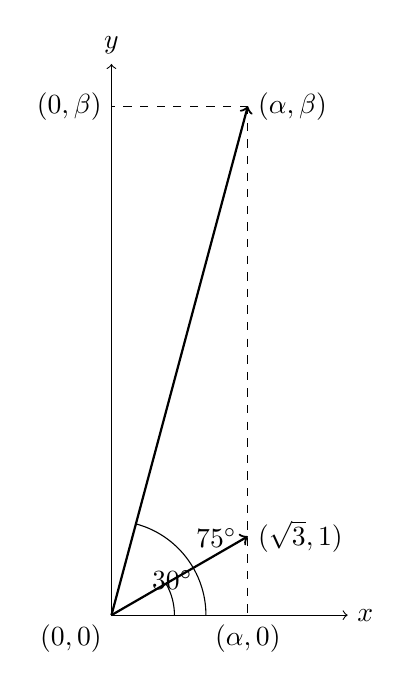
\begin{tikzpicture}
        
        \draw[->] (0,0) -- (3,0) node[right] {$x$};
        \draw[->] (0,0) -- (0,7) node[above] {$y$};
    
        \draw[->, thick] (0,0) -- (1.732,1) node[right] {$(\sqrt{3},1)$};
        \draw[->, thick] (0,0) -- (1.732,6.464) node[right] {$(\alpha, \beta)$};
    
        \draw[dashed] (1.732,6.464) -- (1.732,0) node[below] {$(\alpha, 0)$};
        \draw[dashed] (1.732,6.464) -- (0,6.464) node[left] {$(0, \beta)$};
    
        \draw (0.8,0) arc[start angle=0,end angle=30,radius=0.8] node[midway, above ] {$30^\circ$};
        \draw (1.2,0) arc[start angle=0,end angle=75,radius=1.2] node[midway,above right] {$75^\circ$};
        
        \node[below left] at (0,0) {$(0,0)$};
    
        \end{tikzpicture}
    \end{figure}

    %3rd Question
    \item 
    If for $a>0$, the feet of perpendiculars from the points $\vec{A} \brak{a, -2a, 3}$ and $\vec{B} \brak{0, 4, 5}$ on the plane $lx + my + nz = 0$ are points $\vec{C} \brak{0, -a, -1}$ and $\vec{D}$ respectively, then the length of line segment $\vec{CD}$ is equal to:

    \hfill{\sbrak{\text{Mar 2021}}}
    
    \begin{enumerate}
    \begin{multicols}{4}
        \item $\sqrt{41}$
        \item $\sqrt{55}$
        \item $\sqrt{31}$
        \item $\sqrt{66}$
    \end{multicols}
    \end{enumerate}

    \begin{figure}[H]
        \centering
        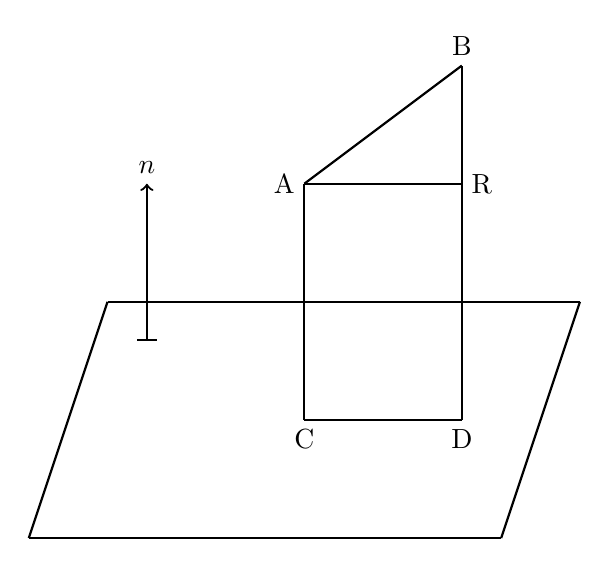
\begin{tikzpicture}
            \draw[thick] (0,0) -- (0,3);
            \draw[thick] (2,0) -- (2,4.5);
            \draw[thick] (0,3) -- (2,4.5);
            \draw[thick] (0,3) -- (2,3);
            \draw[thick] (3.5,1.5) -- (-2.5,1.5);
            \draw[thick] (-3.5,-1.5) -- (2.5,-1.5);
            \draw[thick] (-3.5,-1.5) -- (-2.5,1.5);
            \draw[thick] (3.5,1.5) -- (2.5,-1.5);
            \draw[thick] (0,0) -- (2,0);
            \draw[|->, thick] (-2,1) -- (-2,3);

            \node[below] at (0,0){C};
            \node[left] at (0,3){A};
            \node[below] at (2,0){D};
            \node[right] at (2,3){R};
            \node[above] at (2,4.5){B};
            \node[above] at (-2,3){$\Bar{n}$};
        \end{tikzpicture}
    \end{figure}

    %4th Question
    \item 
    The range of $a \in R$ for which the function 
    \begin{align*}
        f\brak{x} = \brak{4a - 3}\brak{x + \log_e 5} + \brak{a - 7}\cot{\brak{\frac{x}{2}}}\sin^2{\brak{\frac{x}{2}}},
    \end{align*}
    $x \neq 2n\pi$, $n\in\mathbf{N}$ has critical points, is

    \hfill{\sbrak{\text{Mar 2021}}}
    
    \begin{enumerate}
    \begin{multicols}{4}
        \item $\sbrak{-\frac{4}{3}, 2}$
        \item $\lsbrak{1},\rbrak{\infty}$
        \item $\lbrak{-\infty},\rsbrak{-1}$
        \item $\brak{-3, 1}$
    \end{multicols}
    \end{enumerate}

    %5th Question 
    \item 
    Let the functions $f:\mathbf{R}\mapsto\mathbf{R}$ and $g:\mathbf{R}\mapsto\mathbf{R}$ be defined as:
    $f\brak{x}=
    \begin{cases}
        x + 2, & x\leq0\\
        x^2, & x\geq0
    \end{cases}$ \\ and 
    $g\brak{x}=
    \begin{cases}
        x^3, & x<1\\
        3x-2, & x\geq1
    \end{cases}$
    Then, the number of points in R where $\brak{f\circ g}\brak{x}$ is NOT differentiable is equal to: 

    \hfill{\sbrak{\text{Mar 2021}}}
    
    \begin{enumerate}
    \begin{multicols}{4}
        \item $1$
        \item $2$
        \item $3$
        \item $0$
    \end{multicols}
    \end{enumerate}

    %6th Question
    \item
    Let a complex number $z$, $\abs{z} \neq 1$, satisfy $\log_{\frac{1}{\sqrt{2}}} \sbrak{\frac{\brak{\abs{z} + 11}}{\brak{\abs{z} - 1}^2}} \leq 2$. Then, the largest value of $\abs{z}$ is equal to 

    \hfill{\sbrak{\text{Mar 2021}}}
    
    \begin{enumerate}
    \begin{multicols}{4}
        \item $5$
        \item $8$
        \item $6$
        \item $7$
    \end{multicols}
    \end{enumerate}
    
    %7th Question 
    \item 
    A pack of cards has one card missing. Two cards are drawn randomly and are found to be spades. The probability that the missing card is not a spade is:
    
    \hfill{\sbrak{\text{Mar 2021}}}
    
    \begin{enumerate}
    \begin{multicols}{4}
        \item $\frac{3}{4}$
        \item $\frac{52}{867}$
        \item $\frac{39}{50}$
        \item $\frac{22}{425}$
    \end{multicols}
    \end{enumerate}

    %8th Question 
    \item 
    If $n$ is the number of irrational terms in the expansion of $\sbrak{3^{\frac{1}{4}} + 5^{\frac{1}{8}}}^{60}$, then $\brak{n - 1}$ is divisible by

    \hfill{\sbrak{\text{Mar 2021}}}
    
    \begin{enumerate}
    \begin{multicols}{4}
        \item $8$
        \item $26$
        \item $7$
        \item $30$
    \end{multicols}
    \end{enumerate}

    %9th Question 
    \item 
    Let the position vectors of two points $\vec{P}$ and $\vec{Q}$ be $\vec{3\hat{i} - \hat{j} + 2\hat{k}}$ and $\vec{\hat{i} + 2\hat{j} - 4\hat{k}}$ respectively. Let $\vec{R}$ and $\vec{S}$ be two points such that the direction ratios of lines $\vec{PR}$ and $\vec{QS}$ are $\brak{4, -1, 2}$ and $\brak{-2,1,-2}$ respectively. Let lines $\vec{PR}$ and $\vec{QS}$ intersect at $\vec{T}$. If the vector $\vec{TA}$ is perpendicular to both $\vec{PR}$ and $\vec{QS}$ and the length of vector $\vec{TA}$ is $\sqrt{5}$ units, then the modulus of a position vector of $\vec{A}$ is:

    \hfill{\sbrak{\text{Mar 2021}}}
    
    \begin{enumerate}
    \begin{multicols}{4}
        \item $\sqrt{5}$
        \item $\sqrt{171}$
        \item $\sqrt{227}$
        \item $\sqrt{482}$
    \end{multicols}
    \end{enumerate}

    \begin{figure}[H]
        \centering
        \begin{tikzpicture}
            \draw[thick] (-4, -2) -- (4, 2);
            \draw[thick] (-4, 2) -- (4, -2);
            \draw[thick] (0, 0) -- (0, 2);
            \draw[dashed] (0, 0) -- (0, -2);

            \node[below] at (-4, -2){Q};
            \node[above] at (4, 2){S};
            \node[above] at (-4, 2){P};
            \node[below] at (4, -2){R};
            \node[left] at (-0.2, 0){T};
            \node[above] at (0, 2){A};
            \node[right] at (0, 1){$\sqrt{5}$};
        \end{tikzpicture}
    \end{figure}

    %10th Question 
    \item 
    If the three normals drawn to the parabola, $y^2 = 2x$ pass through the point $\brak{a, 0}$ $a \neq 0$, then $'a'$ must be greater than

    \hfill{\sbrak{\text{Mar 2021}}}
    
    \begin{enumerate}
    \begin{multicols}{4}
        \item $1$
        \item $\frac{1}{2}$
        \item $-\frac{1}{2}$
        \item $-1$
    \end{multicols}
    \end{enumerate}

    %11th Question 
    \item
    let  
    \begin{align*}
        S_K = \sum_{r=1}^k \tan^{-1} \sbrak{\frac{\brak{6^r}}{\brak{2^{r+1} + 3^{2r+1}}}}. \text{ Then } \lim_{k\to\infty} S_k = 
    \end{align*}

    \hfill{\sbrak{\text{Mar 2021}}}
    
    \begin{enumerate}
    \begin{multicols}{4}
        \item $\tan^{-1}{\brak{\frac{3}{2}}}$
        \item $\cot^{-1}{\brak{\frac{3}{2}}}$
        \item $\frac{\pi}{2}$
        \item $\tan^{-1}{\brak{3}}$
    \end{multicols}
    \end{enumerate}

    %12th Question 
    \item 
    The number of roots of the equation, $\brak{81}^{\sin^2{x}} + \brak{81}^{\cos^2{x}} = 30$ in the interval \sbrak{0, \pi} is equal to : 

    \hfill{\sbrak{\text{Mar 2021}}}
    
    \begin{enumerate}
    \begin{multicols}{4}
        \item $3$
        \item $2$
        \item $4$
        \item $8$
    \end{multicols}
    \end{enumerate}

    %13th Question 
    \item 
    If $y = y\brak{x}$ is the solution of the differential equation, 
    \begin{align*}
        \frac{dy}{dx} + 2y\tan{x} = \sin{x},
    \end{align*} 
    $y\brak{\frac{\pi}{3}} = 0$, then the maximum value of the function $y\brak{x}$ over $\mathbf{R}$ is equal to :

    \hfill{\sbrak{\text{Mar 2021}}}
    
    \begin{enumerate}
    \begin{multicols}{4}
        \item $8$
        \item $\frac{1}{2}$
        \item $-\frac{15}{4}$
        \item $\frac{1}{8}$
    \end{multicols}
    \end{enumerate}

    %14th Question 
    \item 
    Which of the following Boolean expression is a tautology?

    \hfill{\sbrak{\text{Mar 2021}}}
    
    \begin{enumerate}
    \begin{multicols}{2}
        \item $\brak{p \land q} \land \brak{p \to q}$
        \item $\brak{p \land q} \lor \brak{p \lor q}$
        \item $\brak{p \land q} \lor \brak{p \to q}$
        \item $\brak{p \land q} \to \brak{p \to q}$
    \end{multicols}
    \end{enumerate}

    %15th Question 
    \item let $A = \myvec{\iota&-\iota\\ -\iota&\iota}$.
    Then, the system of linear equations $A^8\myvec{x\\y} = \myvec{8 \\ 64}$ has 

    \hfill{\sbrak{\text{Mar 2021}}}
    
    \begin{enumerate}
    \begin{multicols}{2}
        \item No solution
        \item Exactly two solutions
        \item A unique solution
        \item Infinitely many solutions
    \end{multicols}
    \end{enumerate}

%\end{enumerate}
%\end{document}
